\documentclass[../main.tex]{subfiles}
\rhead{Cameron Eadie}
\begin{document}
 	% Electromagnetic Dust Removal
The Unidentified Falling Objects are likely attracted to the photon beam by the electromagnetic field it generates.
This is based on a number of observations.
The majority of events occur in the vertical plane (see section \ref{UFO_Lit_Review}).
The name "Unidentified Falling Object" was given due to the belief that this uniplanar characteristic was caused by the falling, due to gravity, of macroparticles from the top surface of the beam screen.
However, velocity calculations of UFO events show that they accelerate towards the beam faster than they would under gravity alone.
This characteristic, however, also corresponds to significantly higher surface electric fields found on the beam screen's flat top and bottom surfaces relative to the curved sides.
Also, as investigated in section \ref{chargeAcc}, metallic and polarisable non-metallic (to a lesser degree) particles become negatively charged by a mechanism using the electric field of the proton beam, and non-metallic particles become negatively charged by the electron cloud.
Both kinds of particle would be attracted to the beam and are candidates for UFO events.
It was therefore a natural choice to investigate a variety of electromagnetic field-based mechanisms, by which to clean both metallic and non-metallic UFOs from the beam screen.

%%%%%%%%%%%%%%%%%%%%%%%%%%%%%%%%%%%%%%%%%%%%%%%%%%%%%%%%%%%%%%%%%%%%%%%%%%%%%%%%%%%%%%%%%%%%%%%%%%%%%%%%%%%%%%%%%%%%%%%%%%%%%%%%%%

\section{Dust Levitation}
The first mechanism investigated is a form of active dust mitigation designed for NASA, in order to remove lunar dust from exploration craft, particularly solar panels which are hindered by the presence of such dust on their surfaces. \cite{nasa_dep}.
It uses dielectrophoresis, a phenomenon by which a non-uniform electric field can exert a force on a dielectric particle \cite{esseling_dep}.
Lunar dust comprises of charged and uncharged dust of which the majority is on the scale of micrometres to sub-micrometres, although it is mostly charged due to exposure to solar radiation.
This fits well with the type and size of macroparticles expected inside the LHC, and this dust mitigation mechanism is seen as a possible solution to remove the dust therein. 

\subsection{Mechanism Details} \label{dust_mech}
The proposed dust shield uses a series of long, parallel electrodes connected to a 3-phase AC voltage source.
This induces a dipole moment in any polarisable particles, and then a force is exerted along the direction of the changing electric field.
All particles exhibit dielectrophoretic activity when exposed to electric fields, to some degree.
Metallic particles are polarisable, and some non-metallic particles consist of molecules with an intrinsic dipole moment, allowing them to be polarised.
Some large (greater than \SI{10}{\micro\metre}) particles can also become extrinsically polarised due to movement of surface charge, particularly when they are charged.\\

The dipole approximation for the Dielectrophoretic Force can be derived \cite{green_dep} from the time-independent force equation
\begin{equation} \label{eq:TI_Force}
\textbf{F}(t) = (\textbf{m}(t)\cdot\nabla)\textbf{E}(t)
\end{equation}

where $\textbf{E}(t)$ is the electric field and $\textbf{m}(t)$ is the dipole moment of a spherical particle, which can be expressed in frequency-dependent form as
\begin{equation}
\textbf{m}(\omega) = 4\pi\varepsilon_{m}r^{3}\underline{CM}(\omega)\textbf{E}
\end{equation}

$\underline{CM}(\omega)$ is the Clausius-Mossotti factor which is given by
\begin{equation}
\underline{CM} = \frac{\varepsilon_{p}-\varepsilon_{m}}{\varepsilon_{p}+2\varepsilon_{m}}
\end{equation}

where $\varepsilon_{p}$ and $\varepsilon_{m}$ are the complex permittivities of the particle and the medium respectively. The DEP Force is then given by the real part of equation \ref{eq:TI_Force}
\begin{equation}
\textbf{F}_{DEP} = 2\pi\varepsilon_{m}r^{3}Re(\underline{CM})\nabla|E_{rms}|^{2}
\end{equation}

From this it can be seen that the force experienced by a polarised particle is dependent on the gradient of the electromagnetic field, as well as the real part of the Clausius-Mossotti factor which is comprised of complex permittivities.
By constantly changing the field using AC electrodes of different phases, a traveling wave can be generated which moves the dust along above the surface on which these electrodes are placed.

\begin{figure}[ht]
	\centering
	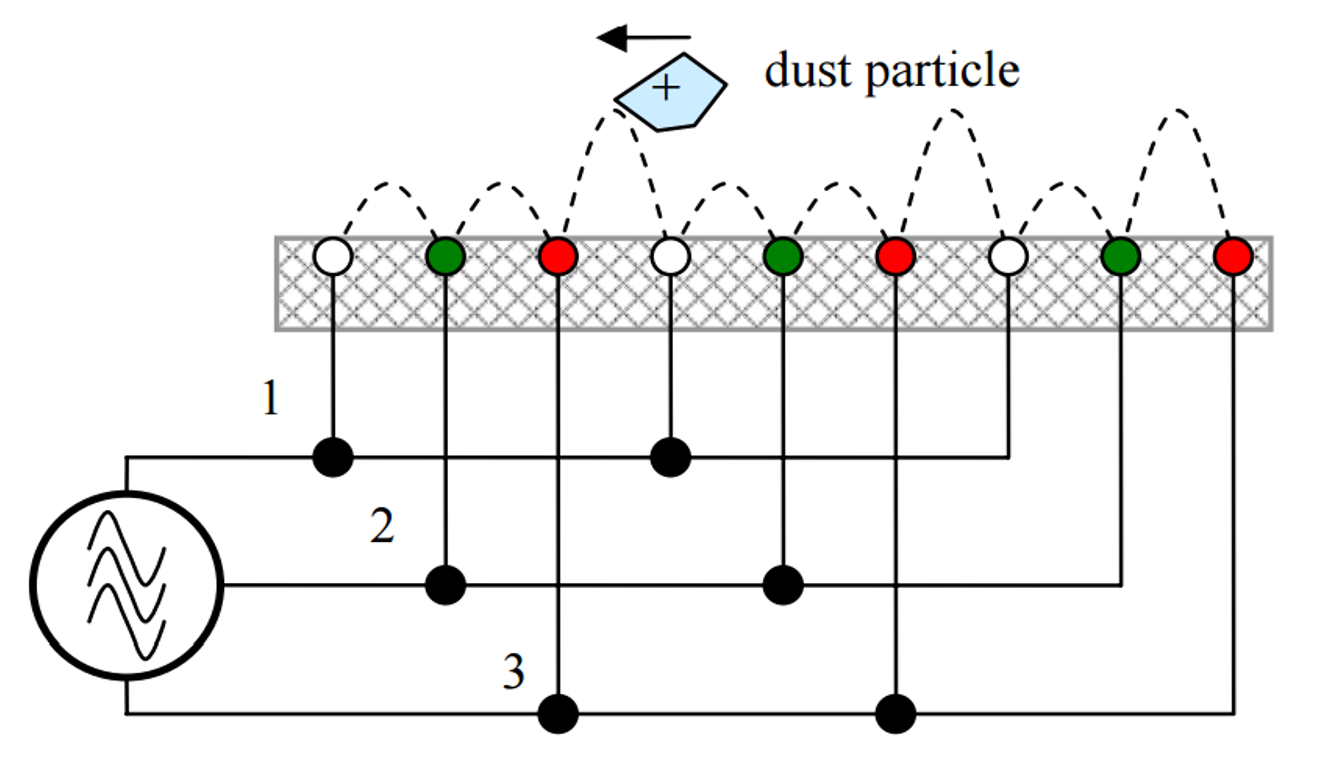
\includegraphics[width=0.8 \textwidth]{DEP_particle.PNG}
	\caption{Three-Phase Electric Curtain \cite{nasa_dep}}
\end{figure}

\subsection{Implementation}
There are two possible ways in which this solution might be implemented.
One possibility is that electrodes would be deployed along the surface of the beam screen, and would then be able to lift and move the dust along the surface of the screen until a point where it could be collected.
The other possibility is to use a craft shaped to travel inside the beam screen.
It could move down the beam pipes with electrodes attached to its surface, and would then be used to move the dust along until it could be collected.
In either case, the electrodes would need to be parallel to the cross section of the beam pipe in order to move the dust along its length.
There are two possible arrangements of these electrodes shown in figure \ref{fig:Electrodes}; three  parallel wires down the length required, with intermittent "fingers" which wrap around the tube, or a continuous spiral design which wraps around the tube without any breaks in the wiring.

\begin{figure}[ht]
\centering
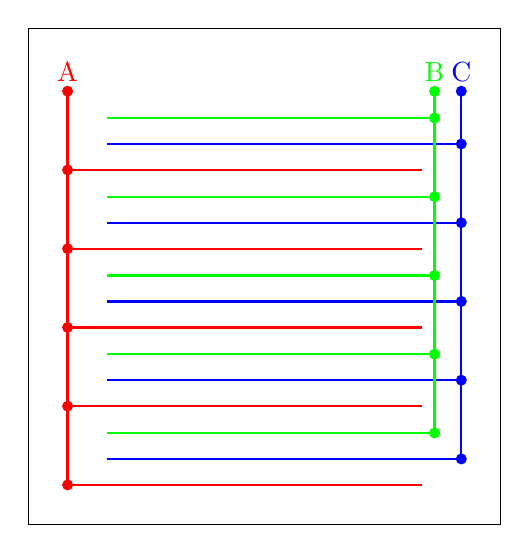
\begin{tikzpicture}
\draw (-0.5,-0.5) -- (5.5,-0.5) -- (5.5, 5.8) -- (-0.5, 5.8) -- (-0.5,-0.5);
\foreach \y in {0,1,...,4} {
	
	\fill[red] (0, \y) circle (0.07);
	\draw[red,thick] (0,\y) -- (4.5,\y);
	
	\fill[blue] (5, \y+0.33) circle (0.07);
	\draw[blue,thick] (5,\y+0.33) -- (0.5,\y+0.33);
	
	\fill[green] (4.66, \y+0.66) circle (0.07);
	\draw[green,thick] (4.66,\y+0.66) -- (0.5,\y+0.66);
	}

\draw[red,thick] (0,5) -- (0,0);
\draw[blue,thick] (5,5) -- (5,0.33);
\draw[green,thick] (4.66,5) -- (4.66,0.66);

\fill[red] (0, 5) circle (0.07) node[above]{A};
\fill[blue] (5, 5) circle (0.07) node[above]{C};
\fill[green] (4.66, 5) circle (0.07) node[above]{B};

  \end{tikzpicture}
  %
  \qquad
  %
  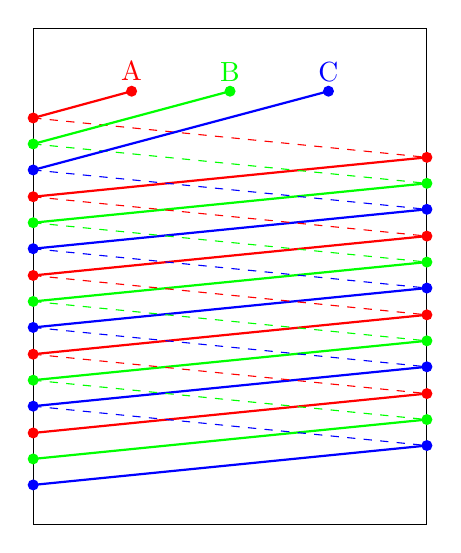
\begin{tikzpicture}
\draw (0,-0.5) -- (5,-0.5) -- (5, 5.8) -- (-0, 5.8) -- (0,-0.5);
\foreach \y in {0,1,...,4} {
	\fill[blue] (0, \y) circle (0.07);
	
	\fill[green] (0, \y+0.33) circle (0.07);
	
	\fill[red] (0, \y+0.66) circle (0.07);
	}
	
\foreach \y in {0,1,...,3} {
	\fill[blue] (5, \y+0.5) circle (0.07);
	\draw[blue,thick] (0,\y) -- (5,\y+0.5);
	
	\fill[green] (5, \y+0.33+0.5) circle (0.07);
	\draw[green,thick] (0,\y+0.33) -- (5,\y+0.33+0.5);
	
	\fill[red] (5, \y+0.66+0.5) circle (0.07);
	\draw[red,thick] (0,\y+0.66) -- (5,\y+0.66+0.5);
}
\foreach \y in {0,1,...,3} {
	\draw[blue,dashed] (0,\y+1) -- (5,\y+0.5);
	
	\draw[green,dashed] (0,\y+1+0.33) -- (5,\y+0.33+0.5);
	
	\draw[red,dashed] (0,\y+1+0.66) -- (5,\y+0.66+0.5);
}

\fill[blue] (3.75, 5) circle (0.07) node[above]{C};
\draw[blue,thick] (0,4) -- (3.75,5);
	
\fill[green] (2.5, 5) circle (0.07) node[above]{B};
\draw[green,thick] (0,4.33) -- (2.5,5);
	
\fill[red] (1.25, 5) circle (0.07);
\draw[red,thick] (0,4.66) -- (1.25,5) node[above]{A};
 \end{tikzpicture}
  %
  \caption{Comparison of Electrode Arrangements (Figure - Tom O'Connor)}
  \label{fig:Electrodes}
 \end{figure}

The spiral design is the simpler of the two designs, and probably easier to apply, however it does have the potential to fail if there is even a single break in one of the wires.
The finger design on the other hand is more complicated, but could be designed so that the main wires are made more robust and potentially protected as they are in a straight line down the pipe/craft, and then failure of individual fingers would not greatly impact the integrity of the whole system.

\subsection{Moving on to Another Mechanism}
This mechanism of dust collection, while promising in some regards, does face a number of issues with implementation.
The series of electrodes need to be installed on the surface of the beam screen or on a robot sent into the LHC.
Installation on the screen surface would require large scale changes to the  inside of the Collider which is unlikely to be approved, and there may be problems with interfering with the electrical properties of the screen.
A robot, on the other hand, would require less excessive alteration to the Collider, and the feasibility of an automated robot is discussed at greater length in section \ref{sec: Feasibility}.
However, due to the levitation mechanism from the electrode-surface, it is not clear whether secondary surface transport (of dust not on the electrode-surface but on a surface opposite) is viable.\\

The UFOs, even if successfully moved along the beam pipe, would then need to be collected.
This calls for the installation of dust collection bins or some other way of removing it, which again would require some sort of changes to the beam pipe.
There is also the question, whether the dust would simply fall through holes in the beam screen when moved, and stay on the bottom inside surface of the beam pipe.
If this were the case, it may still be an improvement, increasing the likeliness of cryotrapping of the UFOs to that surface.
However, due to a number of difficulties, it was decided to move onto another electromagnetic dust removal mechanism, this time one which not only moves the dust, but also removes it permanently from the surface of the beam screen.

%%%%%%%%%%%%%%%%%%%%%%%%%%%%%%%%%%%%%%%%%%%%%%%%%%%%%%%%%%%%%%%%%%%%%%%%%%%%%%%%%%%%%%%%%%%%%%%%%%%%%%%%%%%%%%%%%%%%%%%%%%%%%%%%%%
	
\section{Electrostatic Attraction}
A big issue with a lot of the cleaning mechanisms suggested by this and other groups is that they do not remove UFOs from the inside of the LHC.
They provide ways to remove the macroparticles from the beam screen, or even to move them along its surface, however they still require another step in order to remove them from the Collider.
This is important because it is not clear that simply removing the particles from the surface will solve the problem.
It is therefore preferable to find a mechanism by which the particles can not only be removed from the surface of the beam screen, but one which allows them to then be permanently extracted.
Another advantageous opportunity which this presents is the possibility, if successful, to study the captured UFOs to better understand them.
This means that even if the device does not significantly reduce the number of UFO incidents, it could generate new insight into the problem, which could lead to new ideas about how to proceed.\\

A number of electrostatic and electrodynamic systems were investigated, and the idea which provided the inspiration for the following mechanism is that of an electrostatic precipitator.
Electrostatic precipitators are devices used to remove dust from a flowing gas, such as in coal power stations to remove combustion products from the exhaust fumes.
They use a high electric potential difference between wires in the gas stream, which negatively charge the dust, and the metal plates behind the wires, which then attract the dust to their surface where it stays until it can be disposed of.

\subsection{Mechanism Details}
A charged particle in an electromagnetic field feels a force known as the Lorentz Force
\begin{equation}
\textbf{F} = q\textbf{E} + q\textbf{v}\times\textbf{B}
\end{equation}

where $q$ is the charge of the particle, $\textbf{v}$ is its velocity, and $\textbf{E}$ and $\textbf{B}$ are the electric and magnetic fields respectively.
The magnetic part of the Lorenz Force is of the order of $evB/(m_{proton}m_{particle})$.
This can be neglected to a first approximation for typical UFO velocities $v$ of the macroparticle, even with the high magnetic fields of $B \approx \SI{8.3}{\tesla}$ of the dipole magnets at full energy.
For example, even with a particle speed as high as \SI{1}{\metre\per\second}, the magnetic force is still about 200 times smaller than the electric force on the particle \cite{zimmermann}.
Thus, the  more relevant part of the equation is the first half; a charged particle in an electric field will experience a force due to that field.
This is why negatively charged dust is attracted to the positive potential on the surface of the plates in an electrostatic precipitator, and this idea will be modified in order to remove the dust from the LHC.\\

The proposed mechanism is to have a positively charged plate or surface, which would move down the beam pipe, above the beam screen surface.
The presence of this plate would induce an electric field between itself and the surface of the beam screen, which would cause dust on the screen to become charged (discussed below), and then attract and collect the dust on its surface as it went along, as shown in Figure \ref{fig:DustAttraction}.
The surface would be metallic, however it would be covered with a layer of dielectric.
This would be thin enough so as to not greatly impede the electric field, but thick enough that charge on the attracting surface would not be allowed to flow back into the macroparticles, causing them to be less attracted to the surface and so to fall off.
Similar dust removal mechanisms have been investigated; by IBM for the cleaning of dust from microelectronics during manufacturing \cite{cooper_essc}, by The National Laboratory of High Energy Physics, Oho, Japan, for use in high vacuum systems\cite{saeki_essc}, and by The Fraunhofer Institute for Interfacial Engineering and Biotechnology for use in industrial manufacturing processes \cite{fraunhofer_essc}.

\subsubsection{Metallic and Non-Metallic Dust}
As discussed above, the experiments in the Large Hadron Collider result in the charging of both the metallic and non-metallic particles on the beam screen.
This charging is due to a combination of the electric field from the proton beam and electron cloud generated by electrons which are pulled out of the beam screen.
A charged plate would need to similarly charge particles before they are attracted to it.
In the case of metallic particles, electrons would be attracted to the positive charge of the plate, leaving the beam screen side positively charged.
This would then cause more electrons to flow from the copper surface to neutralise the positive charge and so the particle becomes negatively charged and more likely to be attracted to the plate.
Non-metallic or dielectric dust is more problematic due to the lack of free charge carriers.
Polarisable dust would be polarised similarly to metal particles, and it would also become negatively charged due to surface contact with the copper screen, however there is no continuous influx of negative charge due to the dust's lower conductivity.\\

There is a potential solution to the problem of dust which doesn't become charged enough which was used successfully in experiments by Saeki et al \cite{saeki_essc}.
The way they ensured that particles were negatively charged was by using an electron gun to shower the surface with electrons.
This charges the non-conductive dust's outer surface negatively, and it maintains this charge and so may be picked up due to its low conductivity.
This is similar to the electron cloud mechanism by which we believe similar particles may become charged by the electron cloud in the LHC.

\begin{figure}[ht]
	\centering
	\begin{tikzpicture}[every node/.style={draw,outer sep=0pt,thick}]
	\tikzstyle{spring}=[thick,decorate,decoration={zigzag,pre length=0.3cm,post length=0.3cm,segment length=6}]
	\tikzstyle{damper}=[thick,decoration={markings,  
	  mark connection node=dmp,
	  mark=at position 0.5 with 
	  {
	    \node (dmp) [thick,inner sep=0pt,transform shape,rotate=-90,minimum width=15pt,minimum height=3pt,draw=none] {};
	    \draw [thick] ($(dmp.north east)+(2pt,0)$) -- (dmp.south east) -- (dmp.south west) -- ($(dmp.north west)+(2pt,0)$);
	    \draw [thick] ($(dmp.north)+(0,-5pt)$) -- ($(dmp.north)+(0,5pt)$);
	  }
	}, decorate]

	\tikzstyle{floor}=[fill,pattern=north east lines,draw=none,minimum width=1cm,minimum height=0.3cm]
	\tikzstyle{dielectric}=[fill,pattern=north east lines,draw=none,minimum width=1cm,minimum height=0.3cm]
	\tikzstyle{conductor}=[fill,gray!35,draw=none,minimum width=1cm,minimum height=0.3cm]
	\tikzstyle{dust}=[draw,circle,minimum size=0.15cm]
	\tikzstyle{dustGhost}=[draw, dashed, circle,minimum size=0.15cm]
	\tikzstyle{posCharge}=[draw=none, red]
	\tikzstyle{negCharge}=[draw=none, blue]

	% Floor
	\node (floor1) at (0,0) [floor, minimum width = 6cm] {};
	\draw (floor1.north west) -- (floor1.north east);

	% Dielectric
	\node (dielectric1) at (-0.5,2) [dielectric, minimum width = 3.5cm] {};
	\draw (dielectric1.south west) -- (dielectric1.south east);

	\draw [dielectric] (dielectric1.north west) arc(90:270:0.15) ;
	\draw (dielectric1.north west) arc(90:270:0.15) ;

	\draw [dielectric] (dielectric1.north east) arc(90:-90:0.15) ;
	\draw (dielectric1.north east) arc(90:-90:0.15) ;

	% Conductor
	\node (conductor) at (dielectric1.north) [conductor, minimum width = 4cm, yshift = 0.15cm] {};
	\draw (conductor.south west) -- (conductor.south east);
	\draw (conductor.north west) -- (conductor.north east);

	\draw [conductor] (conductor.north west) arc(90:270:0.15) ;
	\draw (conductor.north west) arc(90:270:0.15) ;

	\draw [conductor] (conductor.north east) arc(90:-90:0.15) ;
	\draw  (conductor.north east) arc(90:-90:0.15) ;

	%Dust
	\node (floordust1) at (floor1.north) [dust, yshift = 0.15cm] {};
	\node (floordust2) at (floor1.north) [dust, yshift = 0.15cm, xshift = -2cm] {};
	\node (floordust3) at (floor1.north) [dust, yshift = 0.15cm, xshift = 0.5cm] {};


	\node (dielectricDust1) at (dielectric1.south) [dust, yshift = -0.15cm, xshift = -0.75cm] {};
	\node (floorGhost1) at (floor1.north) [dustGhost, yshift = 0.15cm, xshift = -0.5cm] {};

	\path[->,>=stealth',red](floorGhost1) edge  [bend left]  (dielectricDust1);

	%Electron Gun
	\begin{scope}[shift={(0,2)},rotate=-35]
	\shade[left color=gray!50!white,right color=gray] (2,3)
	    -- ++(0.8,0) -- ++(-0.15,-1) -- ++(-0.5,0) -- cycle;% column
	  \shade[left color=gray!50!white,right color=gray] (2.2,2)
	    -- ++(0.4,0) -- ++(0,-0.2) -- ++(-0.4,0) -- cycle;% column bottom
	  \draw[gray!80!black] (2,3) -- ++(0.8,0) -- ++(-0.15,-1)
	    -- ++(-0.5,0) -- cycle;%column
	  \draw[gray!80!black] (2.2,2) -- ++(0,-0.2) -- ++(0.4,0)
	    -- ++(0,0.2) node [draw=none](GunBottom) {};%column bottom
	\end{scope}

	\begin{scope}[decoration={snake,amplitude=.4mm,
	        segment length=2mm,post length=1mm}]
	      \draw[decorate,blue,->] (3.0,2.1) --(1.5,0.2);% electron beam
	 \end{scope}
 
	%Positive Charges
	\node (posCharge1) at (conductor) [posCharge, xshift = -1cm] {+};
	\node (posCharge2) at (conductor) [posCharge, xshift = 0cm] {+};
	\node (posCharge3) at (conductor) [posCharge, xshift = 1cm] {+};

	%Negative Charges
	\node (negCharge1) at (floordust1) [negCharge, xshift = 0cm] {-};
	\node (negCharge2) at (floordust2) [negCharge, xshift = 0cm] {-};
	\node (negCharge3) at (floordust3) [negCharge, xshift = 0cm] {-};
	\node (negCharge4) at (dielectricDust1) [negCharge, xshift = 0cm] {-};

	% Labels
	\node[draw=none, xshift = -2cm] (gunLabel) at (-3.5,3.2){Electron Gun (Optional)};
	\node[draw=none, xshift = -4.15cm] (conductorLabel) at (conductor.north west){Conductor};
	\node[draw=none, xshift = -4.45cm] (dielectricLabel) at (dielectric1.south west){Dielectric};J
	\node[draw=none, xshift = -4.2cm] (dustLabel) at (floordust2.north west){Macroparticle};
	

	\path[->,>=stealth'](dielectricLabel.east) edge ([xshift=-0.15cm]dielectric1.west) ;
	\path[->,>=stealth'](conductorLabel.east) edge ([xshift=-0.15cm]conductor.west);
	\path[->,>=stealth'](dustLabel.east) edge (floordust2.west);
	\path[->,>=stealth'](gunLabel.east) edge (3,3.2);

	\end{tikzpicture}
	\caption{Electrostatic Dust Attraction Mechanism (Figure - Tom O'Connor)}
	\label{fig:DustAttraction}
\end{figure}


This mechanism led to over 90\% success rates in picking up non-metallic particles after use of the electron gun, as well as over 90\% success rates for metallic particles without an electron gun.
The gun, therefore, would be a successful solution for non-metallic particles.
It is suspected, however, that the majority of UFOs inside the LHC arc sections are metallic (see section \ref{UFO_Lit_Review}).
In this case it may be a good idea to attempt a solution without the extra complications of an electron gun, and then to return to the possibility if the solution without one is not successful.
The following investigations of a craft do not explore this part of the solution, but it should be kept in mind.

\subsection{Investigation}
\label{ssec:ElectrostaticInvestigation}
The strongest electric field strength experienced by UFOs on the surface of the beam screen is \SI{80}{\mega\volt\per\metre} in the middle of the flat top and bottom parts of the beam screen as noted in section \ref{elecFieldModel}.
However, this field generated by the beam only results in a low rate of UFO events relative to the total number UFOs suggested by the long-term persistence of UFO events throughout operation (see section \ref{UFO_Lit_Review}).
Therefore in order to pick up a large number of UFOs, higher strength electric fields are necessary, and pushing the limits of how strong a field can be generated may lead to the most successful implementation of this method.\\

Calculations were done to calculate the fields used to successfully remove particles from a surface in the experiments by Saeki et al \cite{saeki_essc}.
In this paper, the attractive plate was connected to a voltage source which kept it at a constant voltage of \SI{3}{\kilo\volt}.
It was covered by a thin layer ($d_{1} \approx \SI{0.1}{mm}$) of fiberglass epoxy ($\varepsilon_{r} = 4.4$) and supported over a particle-covered surface in a vacuum, for different particle types and different surface types.
The plate height was then varied, and the success of particle collection calculated using an optical microscope.
The total height range used for metallic particles was \SIrange{3}{6}{\milli\metre}, with a smaller range of \SIrange{4}{6}{\milli\metre} required for some metals (aluminium and iron); however, the larger range is used, especially as this was the range used for copper particles, a highly likely candidate material for UFOs.
For a parallel plate capacitor of this configuration, the electric field is given by
\begin{align}
E &= \frac{V}{\frac{d_{1}}{\varepsilon_{r}} + d_{2}}\\
  &= 0.498 \-- \SI{0.992}{\mega\volt\per\metre} \nonumber
\end{align}

The fields generated are about an order of magnitude greater than those that would be experienced by the UFOs due to the proton beam in the LHC, however this is expected as the intention is to remove the majority of the particles in this experiment, whereas UFO events only happen a few times per hour in the Collider.
It should be noted that these fields up to \SI{1}{\mega\volt\per\metre}, which remove more than 90\% of the particles, establish a field strength which definitely has a particle-removing effect for the majority of particles on a surface.
This means that they can be used as a threshold required for similar screen cleaning in the LHC.
They do not, however, establish a minimum field required, and it is likely that a significant percentage of particles would still be removed by fields below even the lower end of the threshold established here.\\

There are two limiting factors when it comes to generating high strength electric fields.
One factor is the breakdown voltage of the dielectric used to coat the positive plate, as exceeding this will lead to catastrophic dielectric breakdown and damage to the device.
This is a design parameter which can be controlled by choosing the correct material and ensuring it is sufficiently thick to withstand the potential created.
The other factor is the dielectric strength of air.                      
This is a hard constraint on the maximum electric field which can be used, as sparking from the beam screen to the surface of the dielectric could damage it or have other negative consequences, even if the dielectric itself is strong enough.
The dielectric strength of air is \SI{3}{\mega\volt\per\metre} at normal atmospheric pressure \cite{dielectricStrengthAir}.

\subsection{Application of an Electrostatic Force}
Two methods of generating a positively charged surface which would induce an electric field between itself and the beam screen were investigated.

\subsubsection{DC Voltage}
The plate can be connected to the positive terminal of a voltage source, similar to the setup in previous experiments, which results in a constant potential on its surface.
It would then exert a constant electric field between itself and the beam screen, dependent upon the voltage applied and the size of the air gap between the surfaces.
The voltage source would need to be similarly grounded to the beam screen, as an actual connection to form a ground is unlikely.
A plate powered in this way would apply a force of magnitude
\begin{equation}
	F = qE = \frac{V}{\frac{d_{1}}{\varepsilon_{r}} + d_{2}}
\end{equation}

where $V$ is the voltage of the power source, and $d_{1}$ and $d_{2}$ are the thicknesses of the dielectric and the air gap respectively.
Application of experimental results and theory to this method is easier because it is more frequently used, however it has some drawbacks.
In order for there to be a voltage source connected to the plate, either the craft carrying it would have to drag a connective tether behind it down the beam screen, or it would have to carry a battery on board.
A tether would drag along the screen, likely leaving more particles behind than would be picked up.
It also introduces the problem of removing the tether once the craft had traversed the \SI{2.7}{\kilo\metre} length between access points.
A battery on the other hand, adds weight, and may also introduce extra heat into an environment with a fairly restrictive heat budget.

\subsubsection{Stored Charge}
The other alternative is a novel suggestion; using a capacitively charged plate, insulated by the dielectric already present in the design.
This would allow the craft to be self-contained, requiring no additional design implementation once charged.
The charging mechanism would be similar to that of a capacitor, as shown in figure \ref{fig:CapacitiveCharging}.

\begin{figure}[ht]
	\centering
	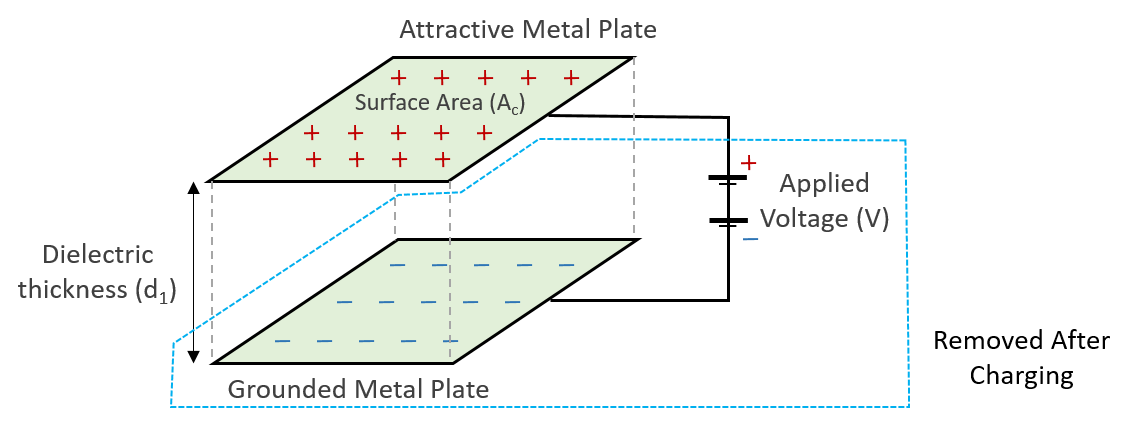
\includegraphics[width=1 \textwidth]{Capacitive_Charging.PNG}
	\caption{Diagram of the Capacitive Charging Mechanism}
	\label{fig:CapacitiveCharging}
\end{figure}

An electrical connection is made to what will be the attractive plate, and a high voltage applied.
At the same time, a ground plate is placed on the other side of the dielectric to form a capacitor.
It then becomes capacitively charged, and this charge is stored, even when the ground plate and electric connection are removed.
After this, the plate will attract particles via the mechanism described above, and as long as it does not lose a large amount of charge, it will continue to attract particles to its dielectric-covered surface.\\

The Capacitance of a parallel plate capacitor is described in terms of its charge-to-voltage ratio, as well as its physical characteristics
\begin{equation}
C = \frac{Q}{V} = \frac{\varepsilon A_{C}}{d_{1}}
\end{equation}

where $Q$ is the charge stored in the capacitor and $V$ is the DC charging voltage.
This can be re-arranged  to form an expression for the charge stored on the surface of the capacitor plates, given in equation \ref{eq:CapacitorCharge}
\begin{equation} \label{eq:CapacitorCharge}
Q = \frac{\varepsilon A_{C}V}{d_{1}}
\end{equation}

When the ground plate and electrical connection are removed, this stored charge will distribute itself evenly around the total surface area of the plate, top and bottom, so $A_{tot} = 2A_{c}$.
This leaves a surface charge density of
\begin{align}
\sigma_{s} &= \frac{Q}{2A_{c}}\\
		   &= \frac{\varepsilon_{o}\varepsilon_{r}V}{2d_{1}}
\end{align}

substituting in equation \ref{eq:CapacitorCharge}.
Then from Gauss' Law it is known that the electric field is given by the ratio of the surface charge density to the permittivity of the medium (air in this case for the part of the field that is of interest), with the permittivity of air ($\varepsilon_{air} = \varepsilon_{o}\varepsilon_{r_air}$) is very similar to that of free space.
This leads to a total force exerted on a charged particle of
\begin{align}
F = qE &= q\frac{\sigma_{s}}{\varepsilon_{air}}\\
	   &= q\frac{\varepsilon_{r}V}{2d_{1}\varepsilon_{r_air}}
\end{align}

This may be weakened by any mirror charges induced in the beam screen.
Calculations and PDE simulations of the complex geometries of the solution craft are investigated at a later point, however it should be noted that in the case of a spherical capacitor plate, the charge will distribute itself only on the outer surface and not on the inner and outer surfaces as it does with a plane capacitor.

\subsection{Implementation}
There is an in-depth study of which craft is best suited for the task of cleaning the UFOs in the LHC in sections \ref{sec: Feasibility} and \ref{sec: Magic Ball - Alex}, however here the two possible implementations are simply introduced, and their technical strengths and weaknesses assessed.
\subsubsection{Automated Device}
A long motorised device fitted to the shape of the inside of the beam screen, so that it might travel down the length of it.
This could utilise either the voltage or charged style of attraction, although the charged style would be less difficult to design for.
The craft device would be automated, moving itself down the tube while attracting dust.

Advantages:
\begin{itemize}
	\item Large surface area of attraction
	\item Charge leakage less likely as no dielectric contact with the beam screen
	\item Potential for inclusion of electron gun
\end{itemize}

Disadvantages:
\begin{itemize}
	\item Heat and dust produced by motors
	\item Potential to get stuck in the LHC
	\item Entry points would need to be modified
	\item Complicated design
\end{itemize}

\subsubsection{Magic Ball}
There is a polycarbonate ball which is passed down sections of the LHC between access points to check for damage to the RF fingers (see figure \ref{fig:RF_Fingers}).
The proposed design is to mimic this ball as much as possible, to ensure that the mechanism is justifiable as completely non-invasive to the current operation of the LHC.
The ball would then be coated internally with a conductor which would store the charge which allows the ball to attract dust to its surface.

Advantages:
\begin{itemize}
	\item Completely self-contained
	\item Uses established method of entry and travel - no modifications to the LHC
	\item Passive dust removal and movement
	\item Relatively easy to design and build
\end{itemize}

Disadvantages:
\begin{itemize}
	\item Potential charge leakage through the contact of resting on the beam screen
	\item Small surface area for dust attraction and storage
\end{itemize}

\section{Summary}
A number of electromagnetic solutions and their variations were investigated to explore the best way to remove UFOs from the beam screen surface in the LHC.
The electrostatic charge mechanism is preferred over the dielectrophoretic force mechanism due to difficulties with the implementation of the latter.
The capacitive charging style of this mechanism provides fewer problems and is a promising idea.
An electron gun addition for non-metallic particle acquisition is discussed but currently discarded for its complexity and for potentially not being necessary.
Two crafts were proposed and their strengths and weaknesses assessed.
A more in depth study follows in sections \ref{sec: Feasibility} and \ref{sec: Magic Ball - Alex}.


\end{document}